\subsection{HF/VHF/UHF Privileges and Sub-bands}
\label{subsec:freq-privs}

When it comes to amateur radio, not all frequencies are created equal—or rather, not all frequencies are accessible to everyone. Depending on your license class (Technician, General, or Amateur Extra), you’ll have different privileges across the HF, VHF, and UHF bands. Think of it like a buffet: the higher your license class, the more dishes you can sample. But even within those bands, there are sub-bands, which are like smaller sections of the buffet table, each reserved for specific modes of operation like CW (Morse code), phone (voice), or digital communications.

\subsubsection*{Frequency Privileges by License Class}
Let’s start with the basics. Technician licensees, while limited in HF privileges, have full access to VHF and UHF bands. On the other hand, General and Amateur Extra licensees enjoy broader access, including more HF bands. For example, Technician licensees can operate phone (voice) on the 10-meter band (28.300–28.500 MHz), while General and Extra licensees can also access the 80, 40, and 15-meter bands for phone operations. 

\subsubsection*{Sub-bands and Mode Allocation}
Sub-bands are like the lanes on a highway—each lane is designated for a specific type of traffic. In amateur radio, sub-bands are allocated for different modes of operation. For instance, the 50.0–50.1 MHz segment is reserved for CW only, while other segments may allow phone or digital modes. This ensures that operators using different modes don’t interfere with each other. It’s like having separate lanes for cars, bikes, and trucks—everyone gets where they’re going without causing a traffic jam.

\subsubsection*{Secondary Service Restrictions}
Sometimes, amateur radio operators share frequency segments with other services, like satellite communications or government operations. In these cases, the Amateur Radio Service is considered a “secondary” user. This means we must avoid interfering with the primary users. If you hear a non-amateur station on a secondary segment, it’s your cue to move to a different frequency. Think of it as being a polite guest at someone else’s party—you don’t want to hog the snacks! (Just move on to get another glass of Sangria!)

\subsubsection*{Avoiding the Edges of Bands}
Ever tried to balance on the edge of a cliff? It’s not a great idea, and the same goes for operating at the edge of a band or sub-band. Transmitter frequency drift, calibration errors, and modulation sidebands can all cause your signal to spill over into restricted areas. To avoid this, it’s best to stay a safe distance from the band edges. This ensures your signal stays where it’s supposed to be, and you don’t accidentally interfere with other services. See Figure~\ref{fig:sidebands} for an illustration of this concept.


\begin{figure}[htbp]
    \centering
    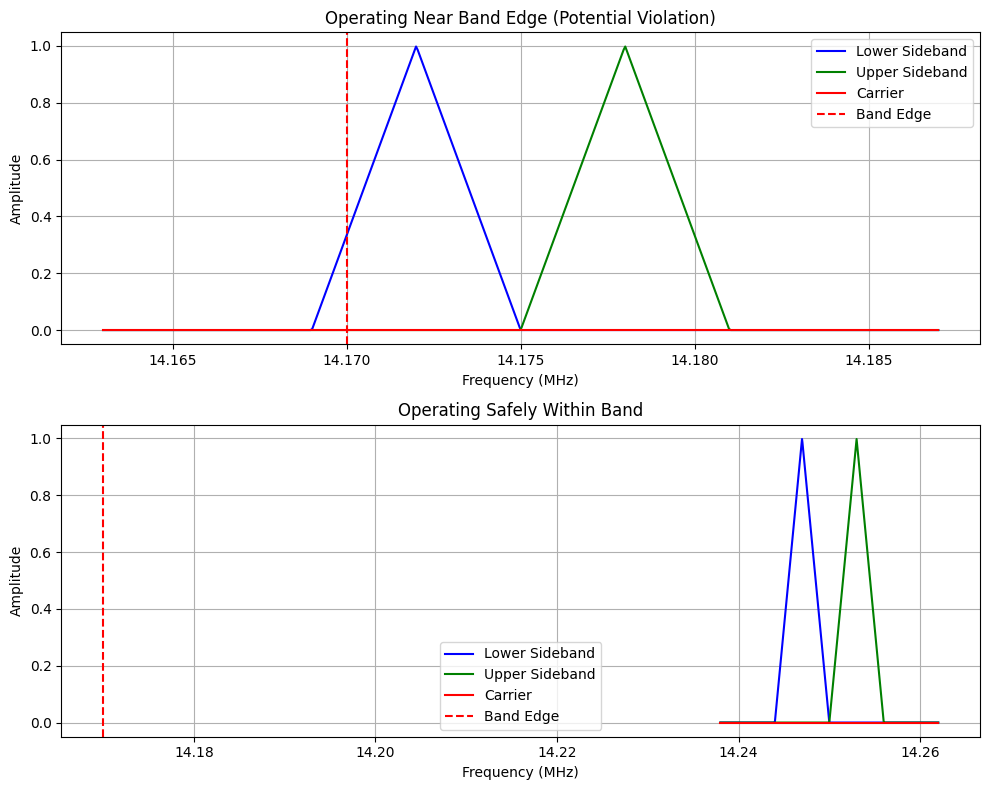
\includegraphics[width=0.8\textwidth]{tech/images/sideband_edge.png}
    \caption{Illustration of Amplitude Modulated (AM) Signal Sidebands and Their Relationship to a Band Edge. The plot depicts two scenarios: (top) a signal operating dangerously close to the lower band edge, with its lower sideband extending beyond the permitted limit; and (bottom) a signal operating safely within the band, with both sidebands contained within the allocated frequencies.}
    \label{fig:sidebands}
    % Prompt: Illustration of modulation sidebands extending beyond the band edge, showing why operating at the edge is discouraged.
    % Software: Matplotlib
\end{figure}


\subsubsection*{Questions}
\begin{tcolorbox}[colback=gray!10!white,colframe=black!75!black,title={T1B01}]
    Which of the following frequency ranges are available for phone operation by Technician licensees?
    \begin{enumerate}[label=\Alph*),noitemsep]
        \item 28.050 MHz to 28.150 MHz
        \item 28.100 MHz to 28.300 MHz
        \item \textbf{28.300 MHz to 28.500 MHz}
        \item 28.500 MHz to 28.600 MHz
    \end{enumerate}
\end{tcolorbox}
Technician licensees have phone privileges on the 10-meter band from 28.300 to 28.500 MHz. The other options fall outside this range.

\begin{tcolorbox}[colback=gray!10!white,colframe=black!75!black,title={T1B02}]
    Which amateurs may contact the International Space Station (ISS) on VHF bands?
    \begin{enumerate}[label=\Alph*),noitemsep]
        \item Any amateur holding a General class or higher license
        \item \textbf{Any amateur holding a Technician class or higher license}
        \item Any amateur holding a General class or higher license who has applied for and received approval from NASA
        \item Any amateur holding a Technician class or higher license who has applied for and received approval from NASA
    \end{enumerate}
\end{tcolorbox}
Any amateur with a Technician class license or higher can contact the ISS on VHF bands. No special approval from NASA is required.

\begin{tcolorbox}[colback=gray!10!white,colframe=black!75!black,title={T1B03}]
    Which frequency is in the 6 meter amateur band?
    \begin{enumerate}[label=\Alph*),noitemsep]
        \item 49.00 MHz
        \item \textbf{52.525 MHz}
        \item 28.50 MHz
        \item 222.15 MHz
    \end{enumerate}
\end{tcolorbox}
The 6-meter band spans 50–54 MHz, so 52.525 MHz falls within this range. The other options are either too low or too high. Another way to remember this is that the product of the frequency (in MHz) and wavelength (in meters) is about 300. So we should be looking for a frequency that is close to 300/6 = 50 MHz. This would eliminate 28.50 MHz and 222.15 MHz. 49.00 MHz is not in the 6-meter band by definition.

\begin{tcolorbox}[colback=gray!10!white,colframe=black!75!black,title={T1B04}]
    Which amateur band includes 146.52 MHz?
    \begin{enumerate}[label=\Alph*),noitemsep]
        \item 6 meters
        \item 20 meters
        \item 70 centimeters
        \item \textbf{2 meters}
    \end{enumerate}
\end{tcolorbox}
146.52 MHz is the national calling frequency for the 2-meter band (144–148 MHz). The other bands don’t include this frequency. We can again use the 300/wavelength rule to infer that 146.52 MHz is in the 2-meter band.

\begin{tcolorbox}[colback=gray!10!white,colframe=black!75!black,title={T1B05}]
    How may amateurs use the 219 to 220 MHz segment of 1.25 meter band?
    \begin{enumerate}[label=\Alph*),noitemsep]
        \item Spread spectrum only
        \item Fast-scan television only
        \item Emergency traffic only
        \item \textbf{Fixed digital message forwarding systems only}
    \end{enumerate}
\end{tcolorbox}
There is no good reason but just because FCC said so.
The 219–220 MHz segment is reserved for fixed digital message forwarding systems. Other modes are not permitted in this segment. (This is a good excuse to get a General license!)

\begin{tcolorbox}[colback=gray!10!white,colframe=black!75!black,title={T1B06}]
    On which HF bands does a Technician class operator have phone privileges?
    \begin{enumerate}[label=\Alph*),noitemsep]
        \item None
        \item \textbf{10 meter band only}
        \item 80 meter, 40 meter, 15 meter, and 10 meter bands
        \item 30 meter band only
    \end{enumerate}
\end{tcolorbox}
Technician licensees have phone privileges only on the 10-meter band (28.300–28.500 MHz). The other bands are either not available or restricted to CW or digital modes.

\begin{tcolorbox}[colback=gray!10!white,colframe=black!75!black,title={T1B07}]
    Which of the following VHF/UHF band segments are limited to CW only?
    \begin{enumerate}[label=\Alph*),noitemsep]
        \item \textbf{50.0 MHz to 50.1 MHz and 144.0 MHz to 144.1 MHz}
        \item 219 MHz to 220 MHz and 420.0 MHz to 420.1 MHz
        \item 902.0 MHz to 902.1 MHz
        \item All these choices are correct
    \end{enumerate}
\end{tcolorbox}
The 50.0–50.1 MHz and 144.0–144.1 MHz segments are reserved for CW only. The other segments allow different modes.

\begin{tcolorbox}[colback=gray!10!white,colframe=black!75!black,title={T1B08}]
    How are US amateurs restricted in segments of bands where the Amateur Radio Service is secondary?
    \begin{enumerate}[label=\Alph*),noitemsep]
        \item \textbf{U.S. amateurs may find non-amateur stations in those segments, and must avoid interfering with them}
        \item U.S. amateurs must give foreign amateur stations priority in those segments
        \item International communications are not permitted in those segments
        \item Digital transmissions are not permitted in those segments
    \end{enumerate}
\end{tcolorbox}
In secondary segments, amateurs must avoid interfering with primary users, which may include non-amateur stations. There’s no requirement to prioritize foreign amateur stations or restrict international communications.

\begin{tcolorbox}[colback=gray!10!white,colframe=black!75!black,title={T1B09}]
    Why should you not set your transmit frequency to be exactly at the edge of an amateur band or sub-band?
    \begin{enumerate}[label=\Alph*),noitemsep]
        \item To allow for calibration error in the transmitter frequency display
        \item So that modulation sidebands do not extend beyond the band edge
        \item To allow for transmitter frequency drift
        \item \textbf{All these choices are correct}
    \end{enumerate}
\end{tcolorbox}
All of these reasons are valid. Operating near the band edge risks interference due to calibration errors, sideband spillover, and frequency drift.

\begin{tcolorbox}[colback=gray!10!white,colframe=black!75!black,title={T1B10}]
    Where may SSB phone be used in amateur bands above 50 MHz?
    \begin{enumerate}[label=\Alph*),noitemsep]
        \item Only in sub-bands allocated to General class or higher licensees
        \item Only on repeaters
        \item \textbf{In at least some segment of all these bands}
        \item On any band if the power is limited to 25 watts
    \end{enumerate}
\end{tcolorbox}
We haven't talked about SSB yet, for now just remember that SSB phone is permitted in at least some segment of all amateur bands above 50 MHz. It’s not limited to repeaters or specific license classes.

\begin{tcolorbox}[colback=gray!10!white,colframe=black!75!black,title={T1B11}]
    What is the maximum peak envelope power output for Technician class operators in their HF band segments?
    \begin{enumerate}[label=\Alph*),noitemsep]
        \item \textbf{200 watts}
        \item 100 watts
        \item 50 watts
        \item 10 watts
    \end{enumerate}
\end{tcolorbox}
Technician licensees are limited to 200 watts PEP on their HF band segments. This ensures they can operate effectively without causing excessive interference.

We will discuss what PEP is in more detail in later chapters.

\begin{tcolorbox}[colback=gray!10!white,colframe=black!75!black,title={T1B12}]
    Except for some specific restrictions, what is the maximum peak envelope power output for Technician class operators using frequencies above 30 MHz?
    \begin{enumerate}[label=\Alph*),noitemsep]
        \item 50 watts
        \item 100 watts
        \item 500 watts
        \item \textbf{1500 watts}
    \end{enumerate}
\end{tcolorbox}
Technician licensees can operate at up to 1500 watts PEP on frequencies above 30 MHz, unless specific restrictions apply (e.g., in certain sub-bands or near band edges).

For maximum power restrictions, see Table~\ref{tab:license_privileges}. Just remember that all licensees can use up to 1500W PEP for any band, except for Technician licensees who are limited to 200W PEP on their HF band segments.